%!TEX root = ./main.tex

\section{One Mental Model}

% SECTION TIMING: 12:00--20:00. The four-part path is the vocabulary anchor for the rest of class.

% Teaching note (45 s): pause before revealing the four-part model.
\begin{frame}{You press Call. What happens next?}
  \begin{columns}[T,onlytextwidth]
    \column{0.42\textwidth}
      \centering
      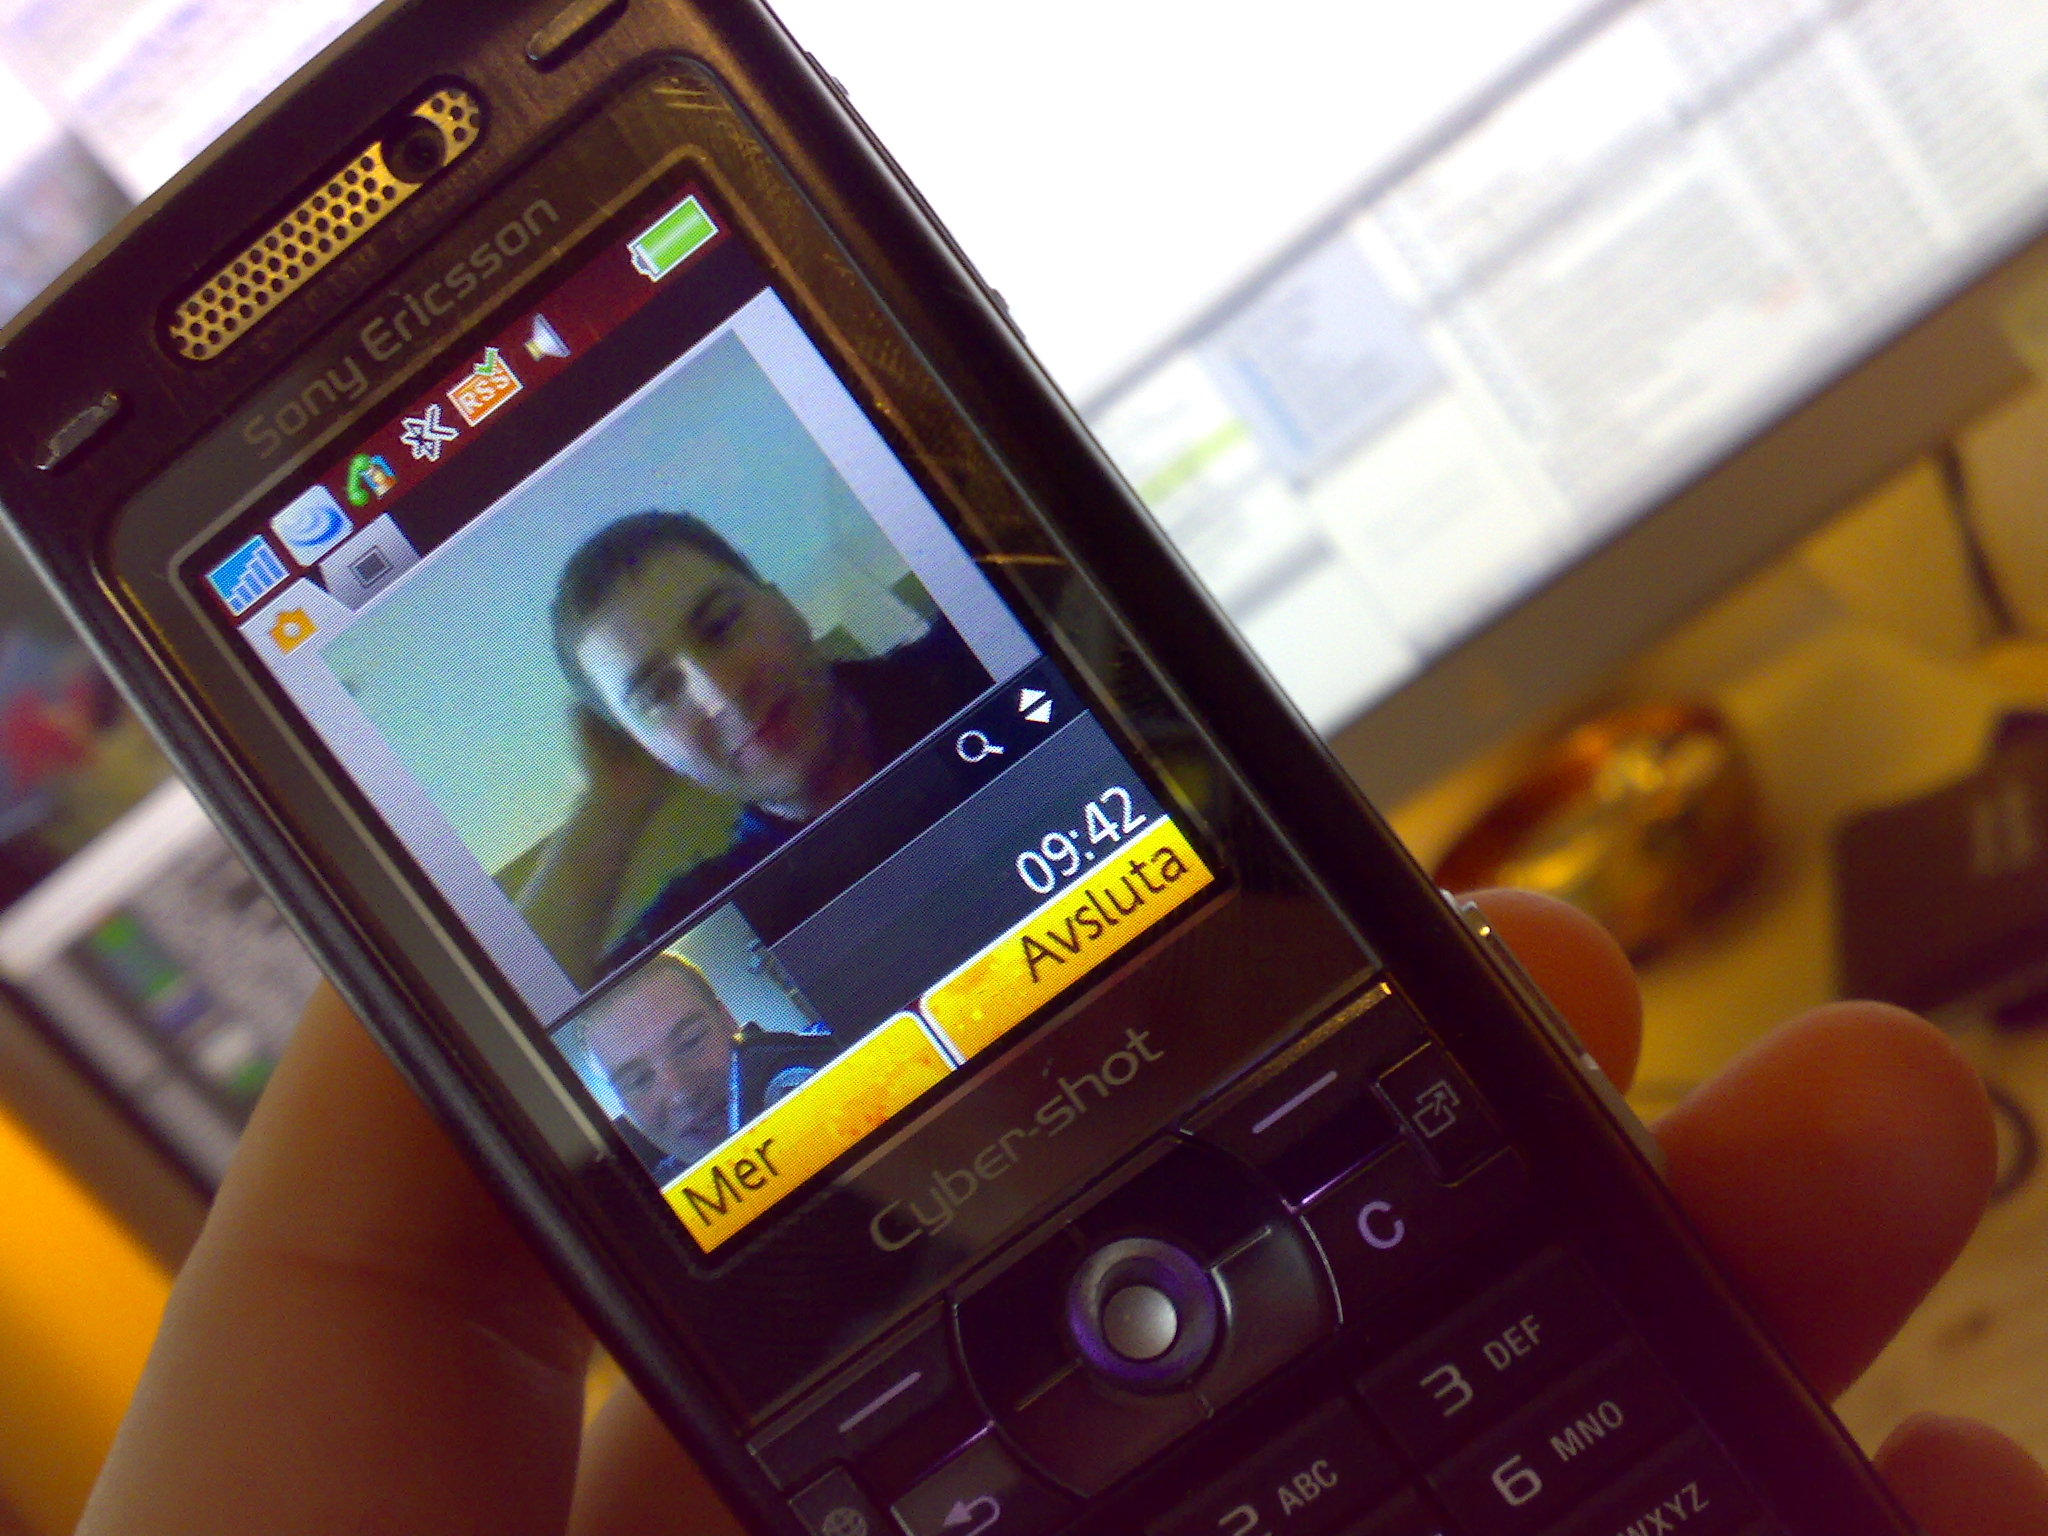
\includegraphics[width=\linewidth]{figure/xg/3g_video_call.jpg}
      \source{https://commons.wikimedia.org/wiki/File:Video_Call.jpg}{UMTS video call}
    \column{0.54\textwidth}
      \large
      Your phone has to find a tower.

      \vspace{0.6em}
      The network has to recognize you.

      \vspace{0.6em}
      Then it has to find the other end.

      \vspace{0.8em}
      \ask{Which part of the network does each job?}
  \end{columns}
\end{frame}

\begin{frame}{Four worlds are hiding behind one tap}
  \centering
  \begin{tikzpicture}[node distance=0.30cm]
    \node[netnode,minimum width=2.0cm,font=\small\bfseries] (ue) {UE\\your device};
    \node[netnode,minimum width=2.2cm,font=\small\bfseries,right=of ue] (ran) {RAN\\radio access};
    \node[corenode,minimum width=2.3cm,font=\small\bfseries,right=of ran] (core) {Core\\control + routing};
    \node[netnode,minimum width=2.6cm,font=\small\bfseries,right=of core] (dn) {PSTN / Internet\\destination};
    \draw[flow] (ue) -- (ran);
    \draw[flow] (ran) -- (core);
    \draw[flow] (core) -- (dn);
  \end{tikzpicture}

  \vspace{1.2em}
  \begin{columns}[T,onlytextwidth]
    \column{0.47\textwidth}
      \Large\textcolor{ranblue}{\textbf{RAN}}

      \normalsize Turns radio waves into managed links.
    \column{0.53\textwidth}
      \Large\textcolor{coreorange}{\textbf{Core}}

      \normalsize Remembers who you are, where you are, and what you may do.
  \end{columns}
  \source{https://www.3gpp.org/technologies/5g-system-overview}{Conceptual model based on 3GPP system architecture}
\end{frame}

\begin{frame}{The network still has the same six jobs}
  \begin{columns}[T,onlytextwidth]
    \column{0.50\textwidth}
      \Large
      \begin{enumerate}
        \item Find a cell
        \item Request access
        \item Prove identity
      \end{enumerate}
    \column{0.50\textwidth}
      \Large
      \begin{enumerate}
        \setcounter{enumi}{3}
        \item Get radio resources
        \item Route voice or data
        \item Move without disappearing
      \end{enumerate}
  \end{columns}

  \vspace{0.8em}
  \takeaway{The node names change. The jobs are surprisingly persistent.}
\end{frame}
